\documentclass[conference]{IEEEtran}
% The preceding line is only needed to identify funding in the first footnote. 
% If that is unneeded, please comment it out.
\usepackage{cite}
\usepackage{amsmath,amssymb,amsfonts}
\usepackage{algorithmic}
\usepackage{graphicx}
\usepackage{textcomp}
\usepackage{xcolor}
\usepackage{hyperref}
\usepackage{tabularx}
\begin{document}

\title{Homework 2 Report - Artificial Neural Networks and Deep Learning}

\author{
Alberto Rota
    \IEEEauthorblockA{ \\
    \textit{Person Code: 10615751}\\
    \textit{Student Number: 964662} \\
    \href{mailto:alberto2.rota@mail.polimi.it}{alberto2.rota@mail.polimi.it}}
\and
Gabriele Santicchi 
    \IEEEauthorblockA{ \\
    \textit{Person Code: 10579046}\\
    \textit{Student Number: 969088}  \\
    \href{mailto:gabriele.santicchi@mail.polimi.it}{gabriele.santicchi@mail.polimi.it}}
\and
Giuseppe Venezia 
    \IEEEauthorblockA{ \\
    \textit{Person Code: 10622477 }\\
    \textit{Student Number: 968395}  \\
    \href{mailto:giuseppe.venezia@mail.polimi.it}{giuseppe.venezia@mail.polimi.it}}
}

\maketitle
\section{Context}
    The goal of this competition is to build a forecasting model that properly 
    predicts the future trends of seven time-series. The available dataset is
    composed of \textit{7} time-series composed by \textit{68528 samples} each. No reference to the sampling frequency is available. 
\section{Preparatory Tasks}
\subsection{Data Loading and Train-Validation Split}
    After uploading the dataset into the environment, the train-validation split has been performed in order to apply the preprocessing function only 
    on the training one. As the amount of samples to be predicted for the challenge is specified, the last \textit{1000 samples} of the 7 time-series 
    has been considered as validation set. 
\subsection{Preprocessing}
    After the train-test splitting, a first inspection has been performed. As it can be seen from Figure \ref{fig:preprocessed_range},
    the time series contain interval with many consecutive flat zones. Regarding the 5th time series, in Figure \ref{fig:pre_processed_5_color}, 
    it can be noticed a huge amount of samples whose mean is largely below the one of the overall time series. Both can be interpreted as a loss of signals that can reduce the performance 
    of the following multivariate forecasting. These reasons led to the ad hoc implementation of two preprocessing functions, whose application results
    can be seen in Fig.3.     Briefly, the first one calculates the derivative among each time series, and if more than 5 consecutive derivative is null, 
    then samples are replaced by NaN values. After that, an ad hoc  symmetric interpolation function has been applied to avoid discontinuity and to replicate 
    the trend of the time series. Results of the symmetric interpolation are shown in Figure \ref{fig:postprocessed_range}.
    The second function gets as hyper parameter a threshold (THR) value, and adds to each samples below the THR the mean of the overall time series over the 
    threshold chosen. Results of this preprocessing step can be observed in Figure in Figure \ref{fig:post_processed_5_color}.
    Both of them have been applied as preprocessing steps in order to observe if the performance of the model would have been increased. 
    \begin{figure}[]
        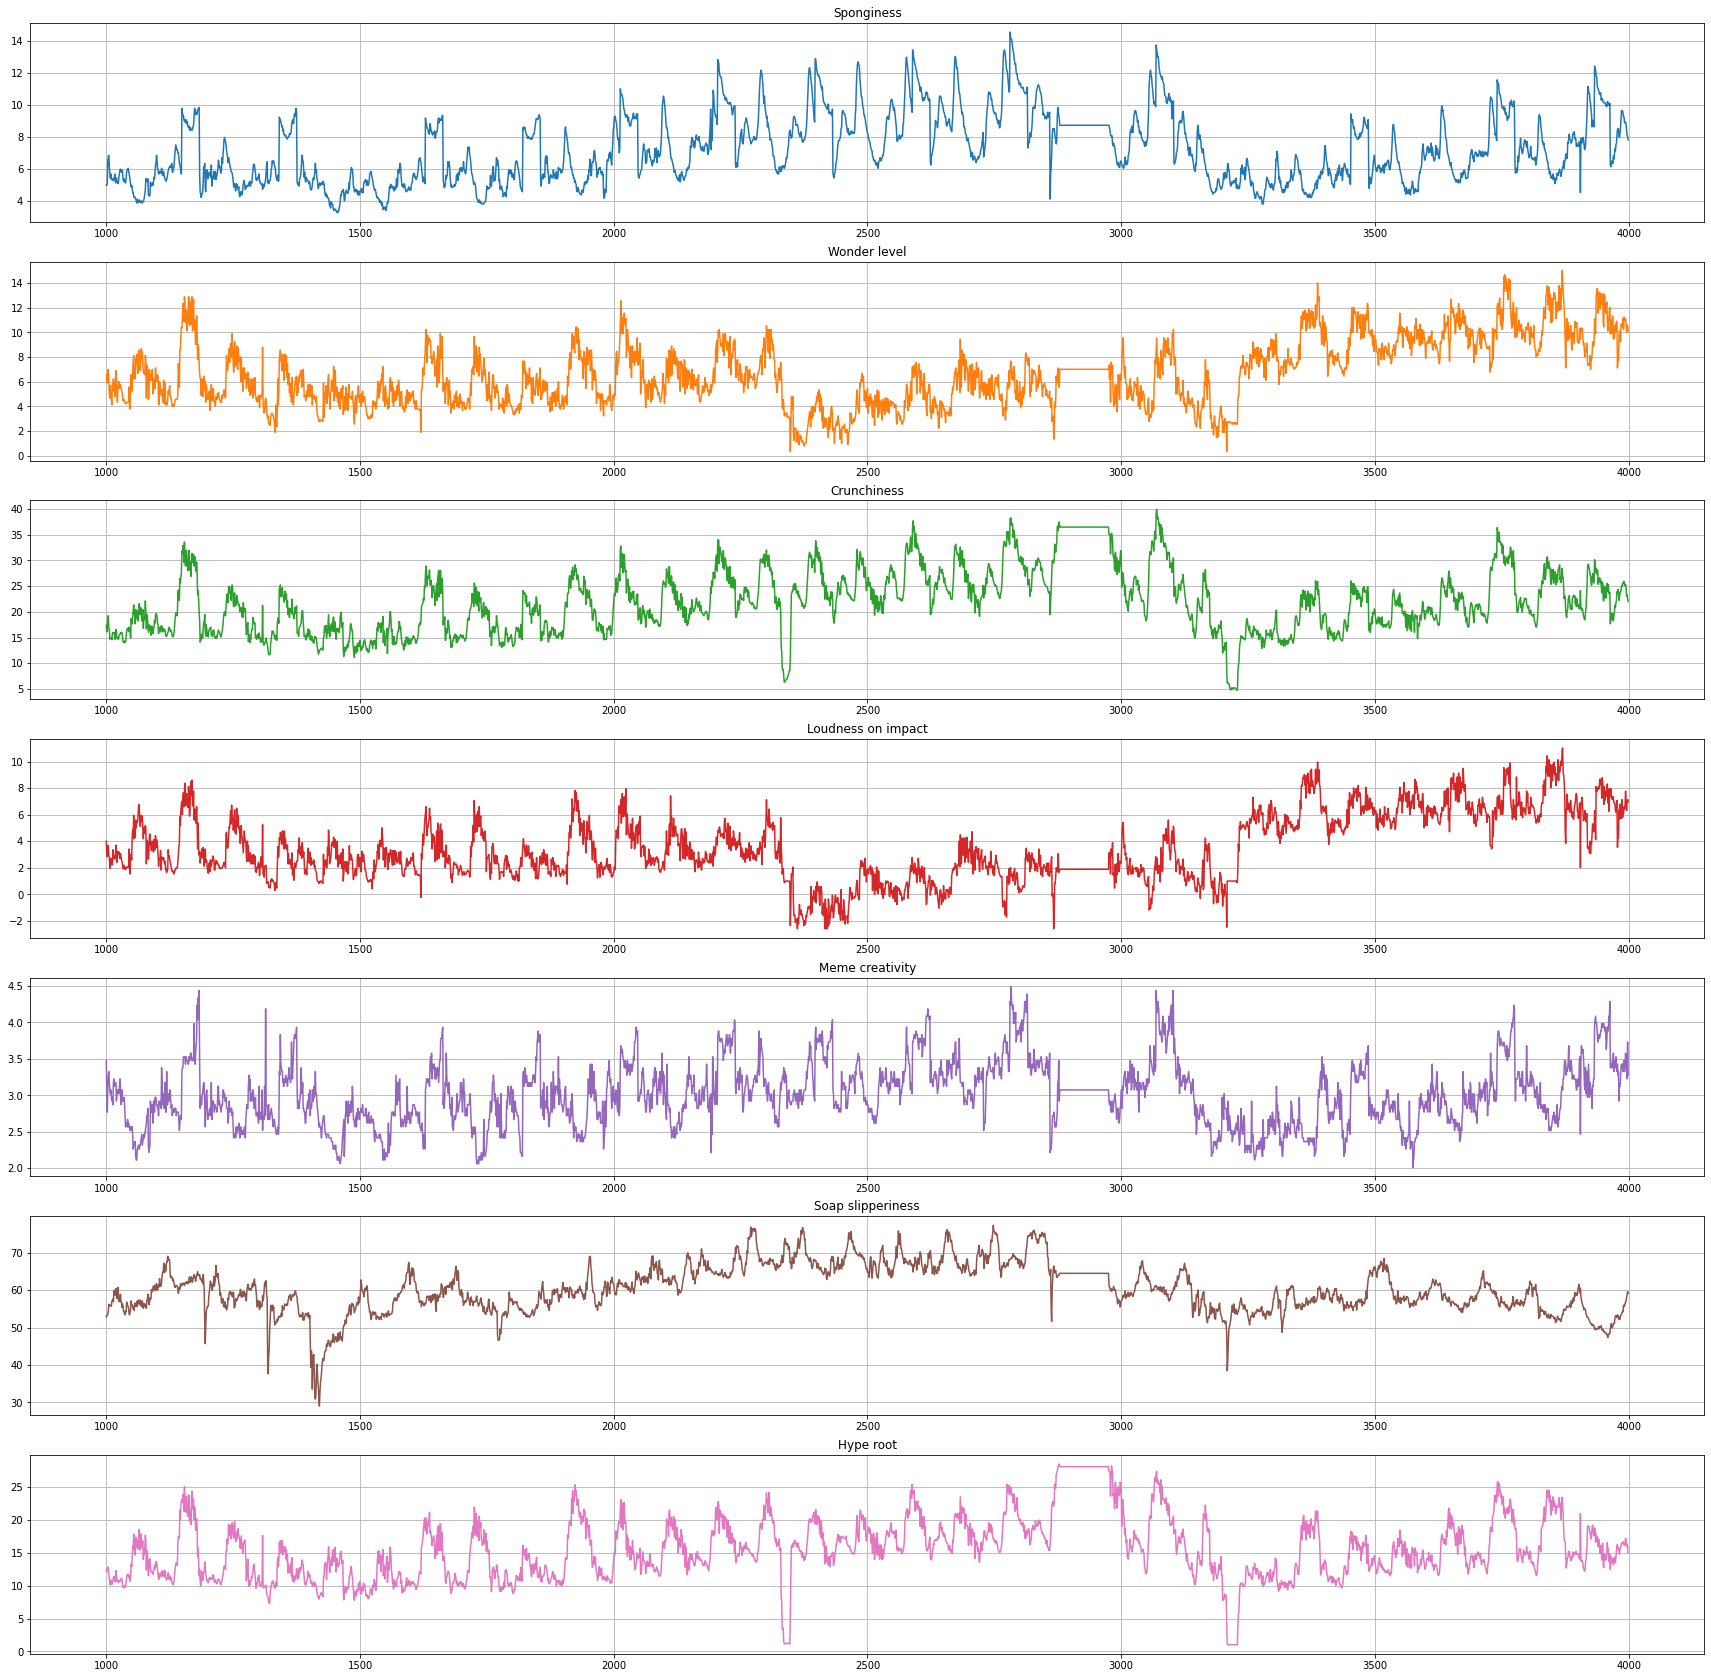
\includegraphics[width=\linewidth]{pre_processed_color.png}
        \caption{Window of the original training dataset}
        \label{fig:preprocessed_range}
    \end{figure}

    \begin{figure}[]
        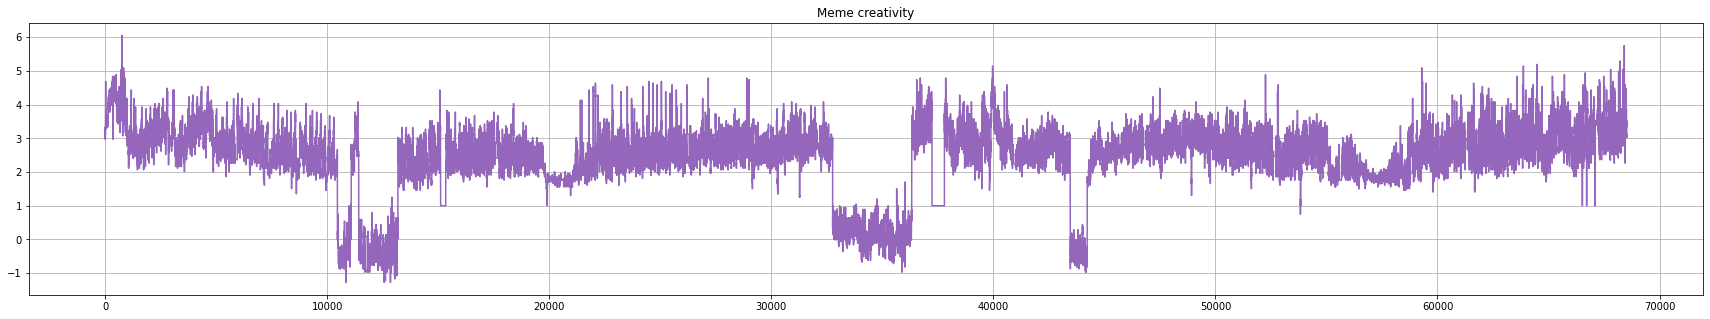
\includegraphics[width=\linewidth]{pre_processed_5_color.png}
        \caption{Window of the training dataset after the symmetric interpolation}
        \label{fig:pre_processed_5_color}
    \end{figure}

    \begin{figure}[]
        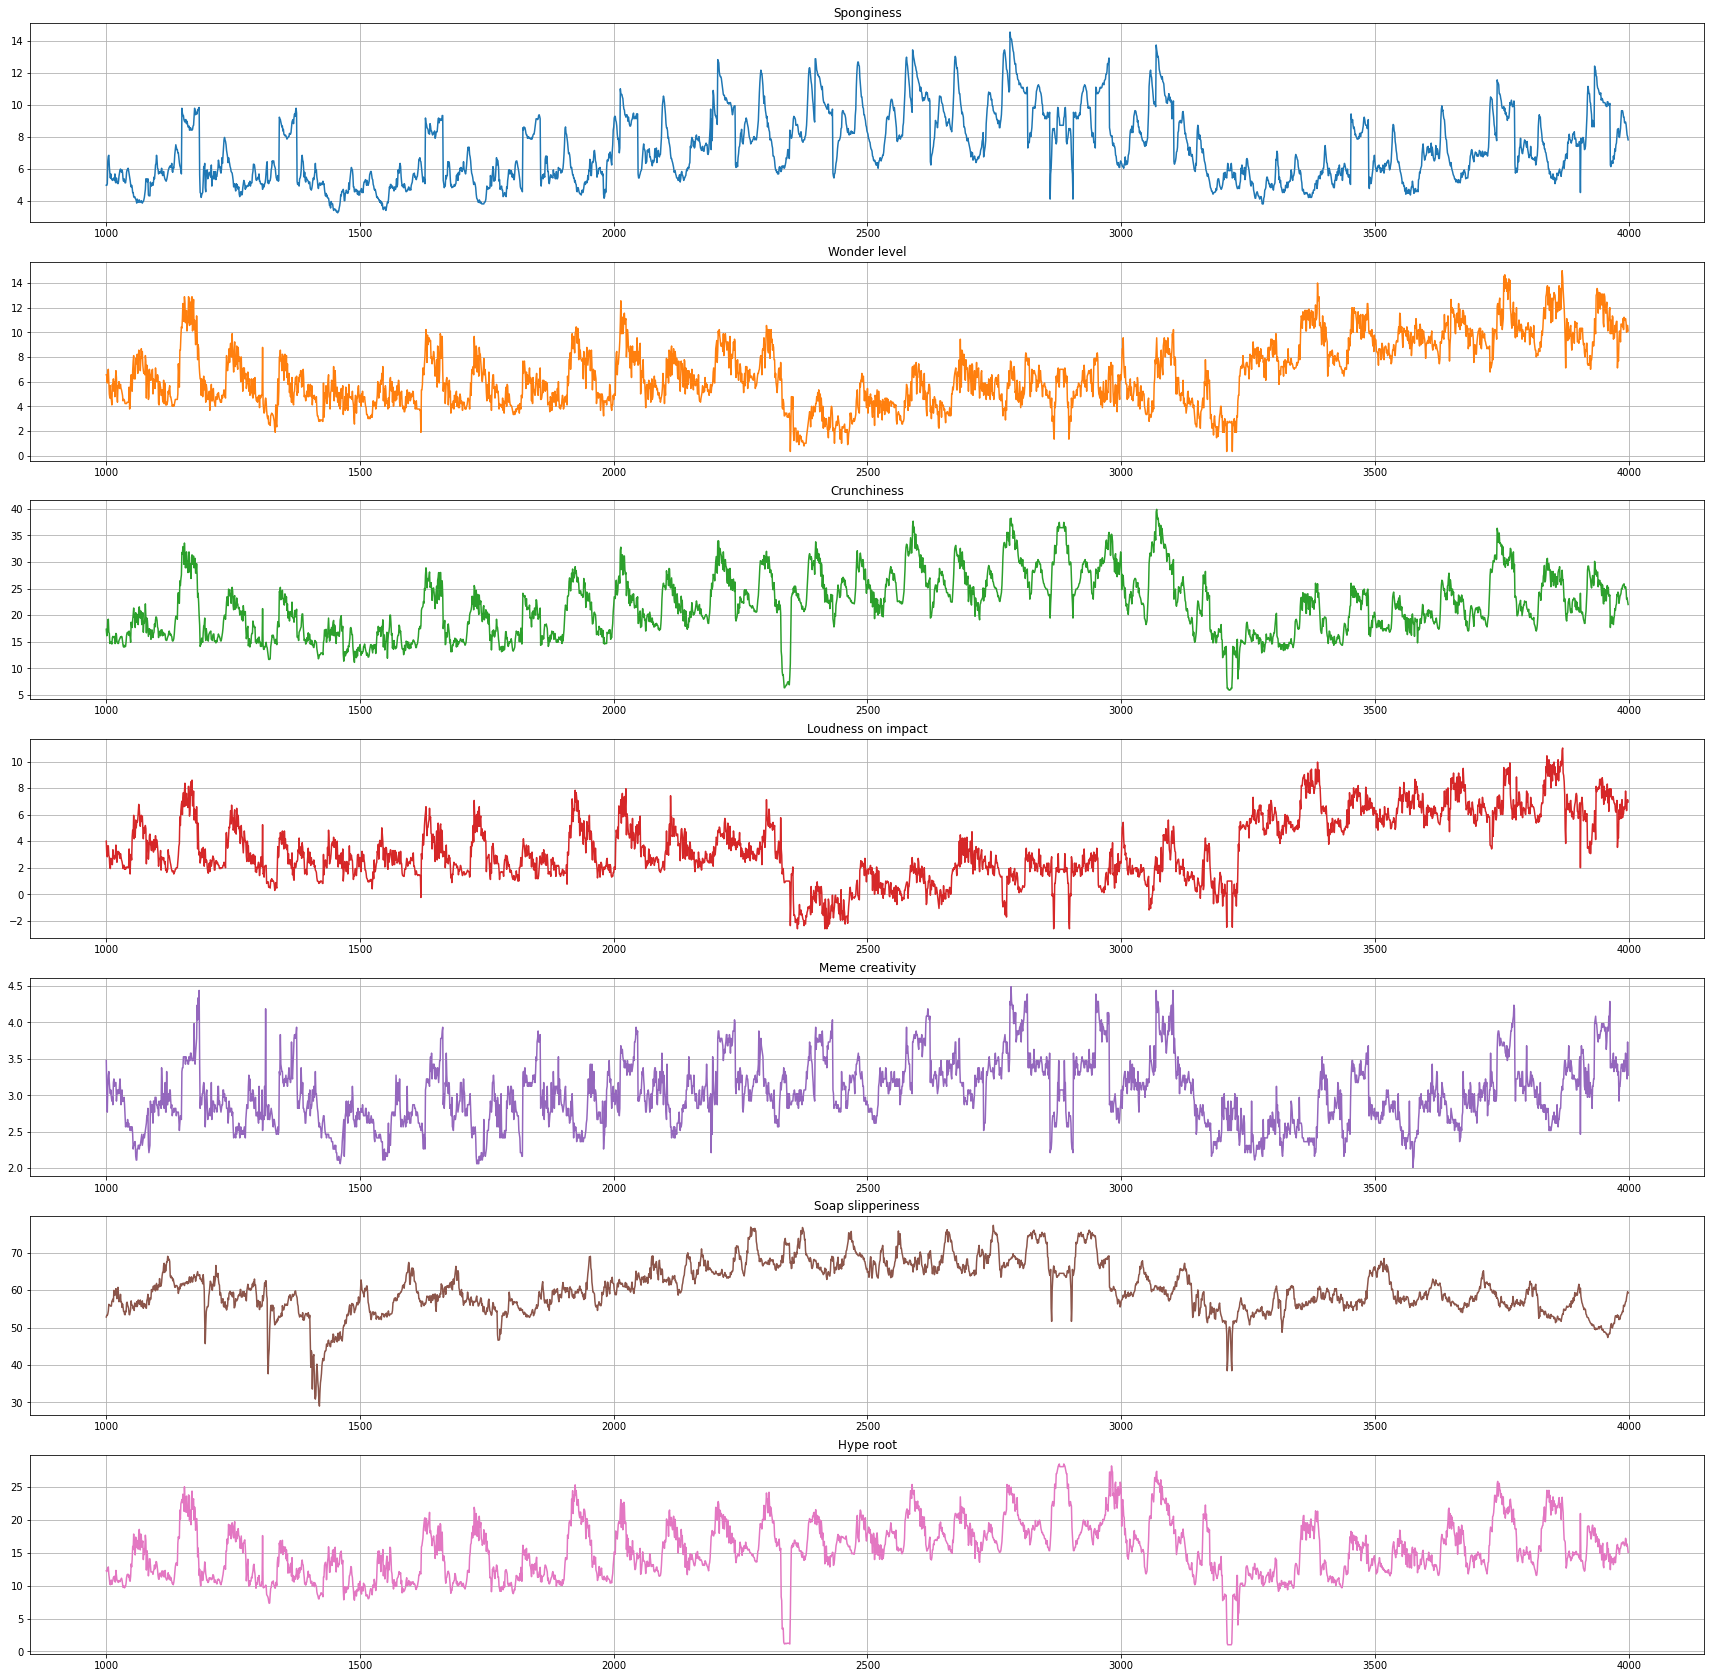
\includegraphics[width=\linewidth]{post_processed_color.png}
        \caption{'meme creativity' time-series before the THR preprocessing step}
        \label{fig:postprocessed_range}
    \end{figure}

    \begin{figure}[]
        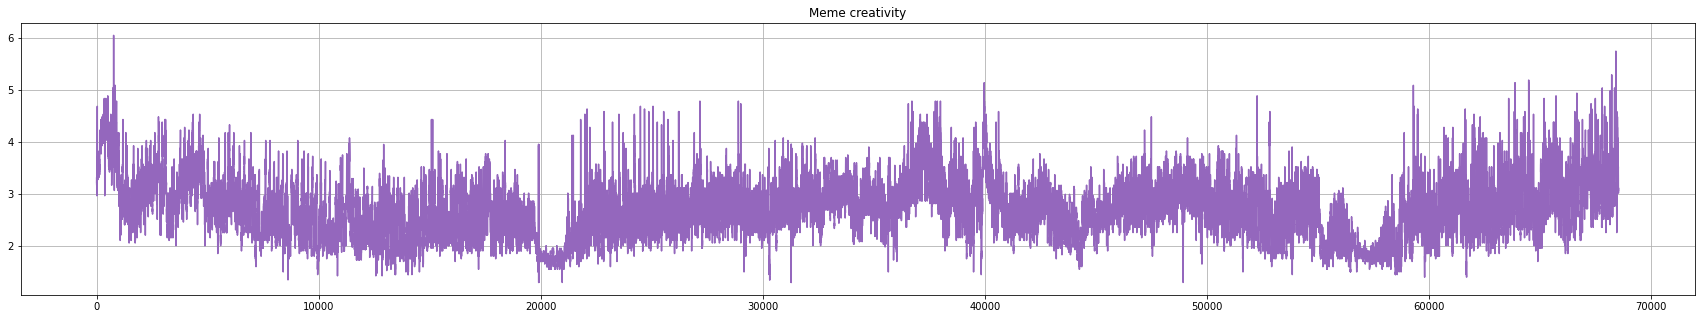
\includegraphics[width=\linewidth]{post_processed_5_color.png}
        \caption{'meme creativity' time-series after the THR preprocessing step}
        \label{fig:post_processed_5_color}
    \end{figure}
\subsection{Normalization}
The last step of the preprocessing consists in the normalization of all the time-series, by means of a min-max approach.

\section{The Model}

\section{Results}


\end{document}